\documentclass[FM,noheader,EN,bwtitles]{tulthesis}
%\documentclass[FM,noheader,EN]{tulthesis}

% Thesis Statement
% Lukas Mateju
% ITE, FM TUL

% use XeLateX to compile

\newcommand{\verze}{1.4}
\usepackage{polyglossia}
\setmainlanguage[variant=american]{english}
\setotherlanguage{czech}
\usepackage{fontspec}
\usepackage{xunicode}
\usepackage{xltxtra}
\usepackage{hyperref}
\usepackage{enumitem}
\usepackage{multirow}
\usepackage{csquotes}

\usepackage[style=authoryear, backend=biber, dashed=false, doi=false, url=false, giveninits=true, uniquename=init, maxbibnames=99]{biblatex}

%\hypersetup{colorlinks=true, linkcolor=tulFM, urlcolor=tulFM, citecolor=tulFM}
\hypersetup{colorlinks=true, linkcolor=black, urlcolor=black, citecolor=tulgray}
%\hypersetup{colorlinks=true, linkcolor=tulgray, urlcolor=tulgray, citecolor=tulgray}
\sloppy

\addto\captionsenglish{%
  \renewcommand{\bibname}{References}%
}
\raggedbottom

\TULtitle{Detekce změny mluvčího s využitím hlubokých neuronových sítí v online vysílání}{Speaker Change Point Detection Based on Deep Neural Networks for Online Streams}
\TULprogramme{P2612}{Elektrotechnika a informatika}{Electrical Engineering and Informatics}
\TULbranch{2612V045}{Technická kybernetika}{Technical Cybernetics}
\TULauthor{Ing. Lukáš Matějů}
\TULsupervisor{Ing. Petr Červa, Ph.D.}
\TULyear{2017}
\TULthesisType{Teze disertační práce}{Thesis Statement}

%\bibliographystyle{references} 
\bibliography{references}
\renewcommand*{\nameyeardelim}{\addcomma\space}
%\DeclareFieldFormat{sentencecase}{\MakeSentenceCase*{#1}}
\titlespacing*{\chapter}{0pt}{-\topskip}{*4}

\begin{document}

\pagestyle{empty}
\ThesisTitle{EN}
\ThesisTitle{CZ}
\pagestyle{plain}
\TULfooternopage
\nofootaddress

\begin{acknowledgement}%[wide]
First and foremost, I would like to express my deepest gratitude to my supervisor, Ing. Petr Červa, Ph.D., for his flawless guidance and continuous support of my Ph.D. study.
Besides my supervisor, I am also grateful to Ing. Jindřich Žďánský, Ph.D. for his thorough insights and endless help.
This work would not be possible without them.
Last but not the least, I'd like to thank my friends \& family and especially Dany for being there for me.

\end{acknowledgement}
\clearpage

\begin{abstractEN}%[wide]

This thesis statement is focused on a task of speaker change point detection for online broadcast streams.
It summarizes the state-of-the-art approaches, explains and sets the motivation and main goals for final thesis and presents the current status of the work.
The proposed approach for speaker change point detection operates in two consecutive phases: speech activity detection and speaker segmentation.
Both phases are heavily discussed within this work.

The proposed speech activity detection approach utilizes deep neural networks as classifier (trained on artificially mixed speech and non-speech signals at desired level of SNR), and context-based weighted finite state transducers as online decoder (to smooth the outputs of DNN).
This approach yields state-of-the-art results on standardized QUT-NOISE-TIMIT dataset, and it is also capable of operating in online mode (i.e., with low latency \& real-time factor).
The proposed speech activity detection approach is now completed, published and fully integrated into TVR monitoring system developed at SpeechLab@TUL, where it saves a significant amount of processing time.

The speaker segmentation approach, similarly to the speech activity detection one, is based on deep neural networks (trained on a mixture of real \& artificial broadcast data) and weighted finite state transducers with forced duration of transition (to determine the change points).
The achieved results on standardized COST278 dataset are promising, but further research is still needed.
A publication is planned for next year.

The final thesis will build on (speech activity detection) and further extend this work (speaker segmentation).  
The final proposed speaker change point detection approach will be then fully integrated into TVR monitoring system developed at SpeechLab@TUL, where it will be utilized to process a large amount of online broadcast streams.

\vspace{0.5cm}
\noindent\textbf{Keywords:}
Deep Neural Networks, Online Application, Speech Activity Detection, Speaker Change Point Detection, Weighted Finite State Transducers.
\end{abstractEN}

%\vspace{2cm}
\clearpage

\begin{abstractCZ}
\begin{czech}
Teze disertační práce se věnují úloze detekce změny mluvčího v online vysílání.
Shrnují současné poznání ve světě, představují motivaci a cíle disertační práce a zabývají se jejím současným stavem.
Metoda pro detekci změny mluvčího, představená v této práci, pracuje ve dvou po sobě jdoucích krocích.
Prvním krokem je detekce řeči, která je následována samotnou detekcí změny mluvčího.
Oběma krokům je věnována vysoká pozornost.

Metoda pro detekci řeči je založená na hlubokých neuronových sítích, které slouží jako klasifikátor, a na vážených konečných stavových transducerech, které vyhlazují výstup ze sítě a zároveň plní roli online dekodéru.
Takto navržená metoda dosahuje nejlepších výsledků na datech QUT-NOISE-TIMIT. 
Je také možné ji bezproblémově nasadit pro online zpracování (nízká latence).
Metoda je považována za dokončenou, byla publikována na mezinárodních konferencích, a dnes je již plně integrována do monitorovacího systému TVR vyvíjeného Laboratoří počítačového zpracování řeči TUL, kde šetří velké množství výpočetního času.


Podobně jako metoda pro detekci řeči je i metoda pro detekci změny mluvčího založená na hlubokých neurnových sítích a na vážených konečných stavových transducerech (tentokrát s pevnou délkou přechodu mezi mluvčími).
Metoda je stále vylepšována, jelikož dosažené výsledky na datech COST278 nejsou plně uspokojující.
První publikace je plánována na příští rok.

Po dokončení se obě metody stanou základním kamenem disertační práce.
Výsledná metoda bude následně začleněna do monitorovacího systému TVR vyvíjeného Laboratoří počítačového zpracování řeči TUL, kde bude využita pro zpracování velkého objemu online vysílání.

\vspace{0.5cm}
\noindent\textbf{Klíčová slova:}
detekce řeči, detekce změny mluvčího, hluboké neuronové sítě, online zpracování, vážené konečné stavové transducery.
\end{czech}
\end{abstractCZ}
\clearpage

\TULfooter
\tableofcontents
\clearpage
\listoffigures

\begingroup
\let\clearpage\relax
\vspace{1.6cm}

\listoftables

\endgroup

\begin{abbrList}
\textbf{BIC} & Bayesian Information Criterion \\
\textbf{CNN} & Convolutional Neural Networks \\
\textbf{DBN} & Deep Belief Networks \\
\textbf{DNN} & Deep Neural Networks \\
\textbf{FAR} & False Alarm Rate \\
\textbf{FER} & Frame Error Rate \\
\textbf{HMM} & Hidden Markov Models \\
\textbf{HTER} & Half-Total Error Rate \\
\textbf{GMM} & Gaussian Mixture Models \\
\textbf{MFCC} & Mel-Frequency Cepstral Coefficients \\
\textbf{MR} & Miss Rate \\
\textbf{SNR} & Signal-to-Noise Ratio \\
\textbf{SAD} & Speech Activity Detection \\
\textbf{SCP} & Speaker Change Point Detection \\
\textbf{SVM} & Support Vector Machines \\
\textbf{RNN} & Recurrent Neural Networks \\
\textbf{RTF} & Real-Time Factor \\
\textbf{VAD} & Voice Activity Detection \\
\textbf{WER} & Word Error Rate \\
\textbf{WFST} & Weighted Finite State Transducers \\
\end{abbrList}

\chapter*{Introduction} 
\label{ch:introduction}
\addcontentsline{toc}{chapter}{Introduction}

Nowadays, a huge amount of audio data is produced every day by television and radio streams as well as other sources.
However, most of this data lacks any kind of labels, which would be useful for a wide range of speech processing applications.
These labels can also carry time marks, which can be further utilized for audio searching, indexing or data retrieval.
Speaker change point detection (often called speaker segmentation) is one of the tasks that can create such labels.
It is a task of finding precise change points between two speakers in a recording.
The output should be labels of speaker homogeneous segments.
Speaker segmentation is usually done without any prior knowledge about the identity or even the number of speakers in recording (i.e., it is treated as a speaker independent task).

Speaker change point detection has many uses as a speech preprocessing task.
In conjunction with speaker clustering, it forms a speaker diarization system.
Speaker diarization focuses on answering the question “who spoke when?”, and the research is driven by challenges held by National Institute of Standards and Technology (NIST).
Speaker change point detection is also a vital part of speaker verification \& identification systems.
It can further be applied for language, gender or emotion detection as well.
The extracted segments can also be used as training data for speaker adaptive approaches to speech recognition.
Lastly, speaker segmentation can be employed for tasks such as audio indexing and retrieval, rich transcription, automatic speech transcription, movie analysis (dialog detection), speaker tracking, multi-speaker detection, etc.

The varied application of speaker change point detection makes it a popular research topic.
Numerous research groups and research centers compete worldwide and propose different approaches in a pursue of state-of-the-art results.
Sometimes, challenges are also being held (e.g. segmentation task by NIST) in an effort to push the field further.
The popularity of this research topic can also be documented by large amounts of accepted papers to international conferences on signal and/or speech processing, such as Interspeech or International Conference on Acoustics, Speech and Signal Processing (ICASSP).
With the recent boom in deep learning in mind, speaker segmentation attracts more and more researchers, and a lot of interesting work should get published in near future.

The remainder of this thesis statement is organized as follows.
In Sect.~\ref{ch:stateOfTheArt}, state-of-the-art approaches to speaker segmentation (and speech activity detection) are summarized as well as an overview of existing systems is presented.
Section~\ref{ch:goalsAndMotivation} explains the motivation behind this thesis and it also sets its main goals.
The current progress of final thesis is in detail discussed in Sect.~\ref{ch:currentStatus}.
Within this section, the proposed speech activity detection and speaker change point detection approaches are presented and their current status is explained as well.
%Within this section, the proposed speech activity detection approach is presented and the current status of proposed speaker change point detection approach is explained.
%The current progress of this work is explained in Sect.~\ref{ch:currentStatus} and the proposed approaches are presented.
%Section~\ref{ch:SAD} is focused on the proposed speech activity detection approach and it forms the main part of this thesis statement.
%The conducted work in speaker change point detection is introduced in Sect.~\ref{ch:SCH}.
Finally, the work is concluded in Sect.~\ref{ch:conclusions}.

%\phantomsection
\chapter{State-of-the-Art}
\label{ch:stateOfTheArt}
%\addcontentsline{toc}{section}{State-of-the-Art}

%The various applications of speaker change point detection make it a popular research topic.
%There is a lot of work published at international conferences every year.
%The challenges held by NIST for speaker diarization also motivate the advances in this field.
%Some of the systems are available for download (with pretrained models) for immediate use as well.

In literature, speaker change point detection is usually carried out in two consecutive phases.
The first phase is speech activity detection, a task of segmenting speech events from non-speech ones.
The extracted speech segments can be optionally further preprocessed by, e.g., gender or language identification.
The latter phase is the speaker change point detection itself. 
During this phase, the final change points between speakers (in extracted speech segments) are found and labeled.

Thanks to the varied application and usefulness of speaker segmentation, there are several fully working systems, which are freely available for download.
Some of them even come with pretrained models for immediate use.

%\phantomsection
\section{Speech Activity Detection}
\label{s:sad}
%\addcontentsline{toc}{subsection}{Speech Activity Detection}

Most of the existing speech activity detection approaches operate in two subsequent stages: feature extraction and speech/non-speech classification.

In the former phase, the classic approaches for feature extraction utilize energy~\parencite{DBLP:conf/interspeech/EvangelopoulosM05}, zero crossing rate~\parencite{DBLP:conf/interspeech/KotnikKH01} or auto-correlation function~\parencite{DBLP:conf/interspeech/GhaemmaghamiBVS10}.
The family of more complex features, which have also been successfully applied, includes MFCCs~\parencite{DBLP:conf/interspeech/SriskandarajaSL15, DBLP:conf/interspeech/RyantLY13}, multi-resolution cochleagram features~\parencite{DBLP:conf/interspeech/ZhangW14}, multi-band long-term signal variability features~\parencite{DBLP:conf/interspeech/TsiartasCKGLSPN13} or channel bottleneck features~\parencite{DBLP:conf/interspeech/Ma14}.
Note that in~\parencite{DBLP:journals/taslp/ZhangW13} features based on the use of deep belief networks have also been proposed.
In practice, various combinations of individual features are usually used to achieve the best possible results.

In the latter phase, various classification algorithms can be used, such as support vector machines~\parencite{DBLP:journals/csl/ShinCK10} or Gaussian mixture models~\parencite{DBLP:conf/interspeech/NgZNMZMVM12, DBLP:conf/interspeech/GhaemmaghamiDKS15}.
In recent years, various deep neural networks architectures started to be employed more and more frequently, including fully connected feed-forward DNNs~\parencite{DBLP:conf/interspeech/RyantLY13}, convolutional neural networks~\parencite{DBLP:conf/interspeech/SaonTSGK13} or recurrent neural networks~\parencite{DBLP:conf/icassp/HughesM13, DBLP:conf/icassp/EybenWSS13}.
More complex approaches, such as jointly trained DNNs~\parencite{DBLP:conf/interspeech/WangDBWDL15} or boosted DNNs~\parencite{DBLP:conf/interspeech/ZhangW14}, have also been proposed.
Moreover, in~\parencite{DBLP:conf/icassp/ThomasSSN15} a combination of DNN and CNN is used.
The output from a given classifier can also be smoothed to further improve the accuracy of the detection.
Recently, various techniques, such as the Viterbi decoder~\parencite{DBLP:conf/interspeech/RyantLY13, DBLP:conf/interspeech/GaoSKHKSN11} or weighted finite state transducers~\parencite{DBLP:conf/interspeech/ChungLL13}, have been applied for this purpose.

Most of the aforementioned works aim primarily at offline applications because applying speech activity detection in an online environment brings further restrictions on the system, such as low computational demands and latency.
The approaches developed namely for the online task include, for example, conditional random fields~\parencite{DBLP:conf/interspeech/GaoSKHKSN11} or accurate endpointing with expected pause duration~\parencite{DBLP:conf/interspeech/LiuHR15}.
Another approach in~\parencite{DBLP:conf/eusipco/MoattarH09} utilizes short-term features.

There is a lack of standardized datasets.
The most utilized one is QUT-NOISE-TIMIT~\parencite{DBLP:conf/interspeech/DeanSVM10} corpus.
Unfortunately, a lot of papers opt for their own data making the comparison of different approaches much harder.

%\phantomsection
\section{Speaker Change Point Detection}
\label{s:scpd}
%\addcontentsline{toc}{subsection}{Speaker Change Point Detection}

Similarly to speech activity detection, speaker change point detection (on extracted speech segments) is usually carried out in two consecutive stages: feature extraction and speaker segmentation itself.
%Similarly to speech activity detection, most of the speaker change point detection approaches operate in two consecutive stages: feature extraction and speaker segmentation itself.

In the first stage, a wide range of features has been utilized over the years.
Simpler features, such as short-time energy~\parencite{DBLP:journals/csl/MeignierMFBB06}, zero-crossing rate~\parencite{DBLP:conf/mm/LuZ02} or pitch~\parencite{DBLP:journals/mms/LuZ05}, were successfully employed.
MFCCs~\parencite{DBLP:conf/interspeech/SinhaTGW05, DBLP:journals/taslp/LuZJ02} are/were probably the most used features even though they were designed for a different task.
Line spectrum pairs (LSP)~\parencite{DBLP:journals/taslp/LuZJ02, DBLP:journals/mms/LuZ05} and perceptual linear prediction cepstral coefficients (PLP)~\parencite{DBLP:conf/icassp/TranterYEW04, DBLP:conf/icassp/ChuTH09} were quite popular as well.
Recently, a focus has shifted to crafting more complex features capturing more speaker specific information.
Nowadays, i-vectors~\parencite{DBLP:conf/icassp/ZhuP16, DBLP:conf/icassp/NeriPRCA17} are the go-to features for most of the state-of-the-art systems.
DNNs have also been used to extract features~\parencite{DBLP:journals/tnn/ChenS11, DBLP:conf/interspeech/YellaS15}.
Novel features, d-vectors, were presented in~\parencite{DBLP:conf/icassp/WangGLXZ17} yielding very good results.
The latest trend are speaker embeddings~\parencite{DBLP:journals/corr/LiMJLZLCKZ17, DBLP:conf/icassp/Bredin17, Jati2017}, which are primarily designed for end-to-end systems.
In practice, the best results are often achieved by a mixture of aforementioned features.

The speaker segmentation approaches can be divided into three main categories: metric-based, model-based and hybrid-based.
The metric-based approaches require a distance measure to be defined first.
After that, two adjacent windows are shifted along the recording, and the distance between them is computed.
If the distance is greater than a predefined threshold, a change point is labeled.
The most commonly used distance measures are Euclidean distance~\parencite{DBLP:conf/mm/LuZ02}, Bayesian information criterion~\parencite{Chen98speaker, DBLP:journals/csl/CettoloVR05}, generalized likelihood ratio~\parencite{150477}, Gaussian divergence~\parencite{DBLP:journals/taslp/BarrasZMG06} and Kullback-Leibler divergence~\parencite{Siegler97automaticsegmentation}.
Support vector machines~\parencite{DBLP:journals/speech/FerganiDH08} were also successfully employed.
On the plus side, these approaches do not require any prior knowledge about the recording (number of speakers, signal characteristics, etc.).
Unfortunately, threshold tuning and frequent consecutive changes in a short span of time are the main obstacles of these methods.
The model-based approaches utilize different models trained from labeled audio data (prior knowledge).
These models are then employed to detect speaker change points when the change from one speaker to another happens.
In literature, the common approaches are HMMs~\parencite{DBLP:conf/odyssey/MeignierBI01} and GMMs~\parencite{DBLP:conf/icassp/Magrin-ChagnolleauRP99, DBLP:journals/taslp/MalegaonkarAS07}.
Eigenvoice-based models~\parencite{DBLP:conf/icassp/CastaldoCDLV08, DBLP:conf/interspeech/DesplanquesDM15} can outperform GMM-based models.
With the recent advances in deep learning in mind, systems based on DNNs~\parencite{DBLP:conf/icassp/Gupta15}, CNNs~\parencite{DBLP:conf/icassp/HruzZ17} and bidirectional long short-term memory RNNs~\parencite{Yin2017} yield state-of-the-art results.
Hybrid-based segmentation approaches combine the metric and model-based approaches to exploit the advantages from both worlds (e.g.~\parencite{DBLP:conf/icassp/MoraruMFBB04}).

The restrictions of applying speaker change point detection in online environment (e.g., low computational demands and low latency) result in significantly lower number of published work.
Furthermore, most of this work has been done for the task of speaker diarization.
The common approaches are based on GMMs~\parencite{4430197, DBLP:conf/interspeech/GeigerWR10, DBLP:conf/eusipco/SoldiBE15}.
In~\parencite{Dimitriadis2017} the authors explored Bayesian information criterion, i-vector features and within class covariance normalization for online application.
The use of i-vectors was also investigated in~\parencite{DBLP:conf/icassp/ZhuP16}.

In literature, there are several commonly used datasets for training and evaluation of speaker segmentation.
One of the first often employed dataset is Hub-4 \parencite{hub-4}.
The French datasets ESTER~\parencite{DBLP:conf/lrec/GallianoGGBMC06}, ETAPE~\parencite{DBLP:conf/lrec/GalibertLACG14} and REPERE~\parencite{DBLP:conf/interspeech/Galibert13} are also commonly utilized.
Speaker segmentation can also be evaluated on multilingual database COST278~\parencite{DBLP:conf/interspeech/ZibertMMMNFGDZPCZKTV05}.
Recently, The Speakers in the Wild dataset~\parencite{DBLP:conf/interspeech/McLarenFCL16} has been published.
Some other worth mentioning datasets are CALLHOME and NIST SRE.
However, most of the published works report the results on only one selected dataset making the comparisons harder.

%\phantomsection
\section{Existing Systems}
\label{s:existingSystems}
%\addcontentsline{toc}{subsection}{Existing Systems}

ALIZE Speaker Recognition toolkit~\parencite{DBLP:conf/icassp/BonastreWM05, DBLP:conf/interspeech/LarcherBFLLLMP13} is an open-source tool primarily designed for speaker recognition.
As such, it also provides support for speaker segmentation (based on HMMs)~\parencite{DBLP:conf/icassp/BozonnetEF10}.
LIUM Speaker Diarization~\parencite{Meignier10liumspkdiarization:, DBLP:conf/interspeech/RouvierDGKMM13} is probably the most known toolkit.
It was originally developed for French ESTER2 evaluation campaign for diarization of broadcast news, and it provides tools for feature extraction (MFCCs), speech activity detection (HMMs), gender detection, speaker segmentation (GMMs, BIC) and speaker clustering.
It also comes with pretrained models for immediate use.
DiarTK~\parencite{DBLP:conf/interspeech/VijayasenanV12} is another toolkit based on GMMs focused on multistream speaker diarization.
Pyannote is a brand new option providing scripts for speech activity detection~\parencite{Yin2017}, speaker change point detection~\parencite{Yin2017} and speaker embeddings (with pretrained models)~\parencite{DBLP:conf/icassp/Bredin17}.
It is based on long short-term memory recurrent neural networks, and it yields very promising results.
Newly, speaker segmentation based on deep neural networks is being worked on to be added to Kaldi toolkit~\parencite{Povey_ASRU2011}.

Other notable systems, such as CMU Segmentation toolkit, AudioSeq or SHoUT toolkit, can be utilized as well, but their performance is usually outperformed by new counterparts.

%\phantomsection
\chapter{Motivation and Goals}
\label{ch:goalsAndMotivation}
%\addcontentsline{toc}{section}{Motivation and Goals}

The recent advances in deep learning resulted in a novelty approach to speech recognition~\parencite{DBLP:journals/taslp/DahlYDA12}, which yielded state-of-the-art results by a large margin over the previously conventional approaches.
This success provoked further research of deep neural networks and their application to a different range of application.
In case of this thesis, it is for the task of speaker change point detection.

SpeechLab (Laboratory of Computer Speech Processing) of Technical University of Liberec (TUL) has been focusing on speech processing and speech recognition for a long time.
The TVR monitoring system developed here at SpeechLab@TUL carries out 24/7 transcription of radio and TV broadcasts in a range of different languages.
In peak hours (during the day), it transcribes up to 120 streams in parallel in real-time.
During the non-prime hours (mostly in night), it is still processing at least 20 online streams every second.
The day average ranges from 60 to 80 simultaneously transcribed online streams.
Approximately 133 days (3,196 hours or 75GB) of recordings are being processed every day.
%Last month, approximately 4,130 days (99,100 hours or 2.3TB) of recordings were transcribed in processing time of 1,333 days (32,000 hours).
%These number demonstrate the capability of the system to operate in real-time without any issues.
The biggest chunk of every day transcribed streams form Polish (80 broadcasts monitored), Czech (47) and Slovak (12) broadcasts.
However, a wider range of Slavic languages, such as Russian (approximately 20 broadcast monitored), Bulgarian (20), Croatian (10) or Serbian (10) and more, are being transcribed as well.
%The system also supports additional languages including Swedish or English and there is more to come. 

An integration of speaker change point detection approach (operating in two consecutive phases: speech activity detection and speaker segmentation) to this existing system would be beneficial to SpeechLab@TUL for many reasons.
Firstly, speech activity detection would be used as a preprocessor for online streams to run the transcriber only on speech segments.
This should result in significant reduction in processing time, and it should ease the CPU load as well (if the stream contains a lot of non-speech segments (e.g. music radios)).
It should also yield a better accuracy of transcriptions as the non-speech parts are omitted from being transcribed.
Secondly, the detected speech segments would be used as inputs to speaker segmentation to find transitions between two speakers.
The created labels would ease the handling of online streams as it would provide additional information, and it would segment the streams to smaller speaker homogeneous chunks, which could be easily further utilized.
These chunks form a good starting point for a full diarization system, which could be then extended to speaker verification \& identification systems to provide the transcribed recordings with even more  valuable information.
The detected segments could also be used as training data for future speaker adaptive approaches to speech recognition.
Lastly, SpeechLab@TUL is always trying to improve the TVR monitoring system with additional functionality, especially based on state-of-the-art-technologies, and is planning to do so in future as well.
Speaker segmentation is considered as one of the wanted additional functionality.

An integration of any of the existing systems (see Sect.~\ref{s:existingSystems}) would be a tough task as they are not a very good fit for the requirements of SpeechLab@TUL.
They are quite often fine-tuned to very specific conditions (telephone conversations, broadcasts (French - LIUM Speaker Diarization), etc.), which may or may not be suitable for TVR monitoring system. However, it would most likely result in a need of training new models on proper data.
%On plus side, the pretrained models of LIUM Speaker Diarization were tuned on French broadcasts.
Nextly, except for Pyannote, which was released recently in 2017, all of the systems are built on overcome technologies (mostly GMM-based), and they do not yield state-of-the-art results.
An approach based on deep learning would fit philosophy of SpeechLab@TUL more as the transcriber is based on deep neural networks as well.
And most importantly, none of the systems is primarily designed for online use.
The required input is an audio file or a parametrized signal, and some of the systems even require multiple passes through data (e.g. LIUM Speaker Diarization).
A lot of additional work would be needed to get the systems functioning for online streams.
It might not even be possible for some systems.
Lastly, the TVR monitoring system is a distributed application.
As such, it is distributed in a docker image.
This brings further requirements, such as good scalability or fast and stable implementation.
These facts result in a need of speech change point detection approach developed specifically for the TVR monitoring system.

%An integration of any of the existing systems (see Sect.~\ref{s:existingSystems}) would be tough as they are not a very good fit for the requirements of SpeechLab@TUL.
%They are quite often fine-tuned to very specific conditions and most of them are built on overcome technologies.
%Most importantly, they are usually not primarily designed for online use as well.
%This results in a need for a speech change point detection approach developed specifically for the TVR monitoring system.

%SpeechLab (Laboratory of Computer Speech Processing) of Technical University of Liberec focuses on speech recognition and speech processing for a long time.
%This makes speaker change point detection an interesting task for SpeechLab for many reasons.
%Firstly, a substantial amount of data of various Slavic languages is being transcribed here every day.
%Speech activity detection can filter the non-speech parts out to save the processing time and to improve the accuracy of the system.
%Secondly, a language identification can distinguish between Slavic languages and choose correct acoustic and language models for speech recognition.
%It could also be used to mine more training data for low-resource languages.
%Lastly, speaker change point detection can be used to find speaker homogeneous segments, which can be easily further utilized.
%It is a good starting point for a full diarization system which could be then extended to speaker verification \& identification systems to provide the transcribed recordings with additional valuable information.
%The segments could also be used as data for future speaker adaptive approaches to speech recognition.
%It is also crucial that the speaker change point detection system operates with online streams as nowadays most of the work in SpeechLab is designed for online use.

The main goal of this work is thus to develop a speaker change point detection approach that:
\begin{enumerate}
	\item utilizes state-of-the-art techniques including namely DNNs,
	\item yields at least comparative results with already existing methods,
	\item operates in two or more consecutive phases, where the first one allows for robust speech/non-speech detection,
	\item operates in an online mode with a low latency in order to process real-time streams,
	\item can be integrated into an existing TVR monitoring system developed at SpeechLab@TUL.
\end{enumerate}

%The goals of the thesis and the speaker change point detections system itself could be summarized as:
%\begin{itemize}
%	\item The system should be based on state-of-the-art technologies, such as deep neural networks and weighted finite state transducers.
%	\item A speech activity detection module should be designed to separate speech/non-speech segments.
%	\item An optional language identification module could be crafted to distinguish between Slavic languages.
%	\item A final speaker change point detection module should be implemented to find precise transitions between speakers.
%	\item The system should be able to operate in real-time with low latency to segment online streams.
%	\item The results should be highly competitive.
%\end{itemize}	

%It is important to note that the goals of this thesis were set up before the recent boom in deep learning.
%The advances as shown in previous section confirm the importance and usefulness of the topic.
%This can also be confirmed by author's accepted papers on topic~\parencite{SIGMAP16, ICASSP17, SPRINGER17} and on use of DNNs in slightly different field of study~\parencite{ECMSM15, TSP16, TSD16, TSD17} at international conferences.
%The research in this field is also very much alive as the amount of corresponding papers at recent Interspeech or ICASSP conferences shown.
%The research in this field is also very much alive as the amount of corresponding papers at recent Interspeech~\parencite{DBLP:conf/interspeech/2016} or ICASSP~\parencite{DBLP:conf/icassp/2017} conferences shown.

%\phantomsection
\chapter{Current Status}
\label{ch:currentStatus}
%\addcontentsline{toc}{section}{Current Status}

The final thesis is still a work in progress.
The progress can be divided into two successive tasks as the proposed speaker change point approach operates in two consecutive phases as well:

%As the proposed speaker change point detection approach should operate in two consecutive phases, the progress can be monitored in them as well.
%The proposed speaker change point detection approach should operate in two consecutive phases.
%The progress can be thus observed in two phases as well: 
%The progress can be observed in two consecutive phases:
%It can be divided into two main observable subtasks: 

\begin{itemize}
	\item Speech Activity Detection - \textbf{completed and published}
	%The speech activity detection approach is fully completed and published.
	
	%It is mainly based on feed-forward deep neural networks and weighted finite state transducers.
	%The DNN is used as a speech/non-speech classifier while the context-based WFST smooths the outputs.
	%This design yields state-of-the-art results in low and medium noise conditions on standardized QUT-NOISE-TIMIT dataset.
	%It is also suitable for online use as it operates with low latency as well as real-time factor.
	
	%The initial research introducing the main idea and basic smoothing model was presented in~\parencite{SIGMAP16} at SIGMAP 2016 held in Lisbon.
	%The improved context-based smoothing model which yields state-of-the-art results was introduced in~\parencite{ICASSP17} at ICASSP 2017 conference in New Orleans.
	%Finally, an extended version of this work presenting more experiments and in detail evaluation on QUT-NOISE-TIMIT was published in~\parencite{SPRINGER17}.
	%The papers also report the improvements of employing proposed speech activity detection approach in conjunction with speech recognizer.

	%\item Language Identification - \textbf{in progress}
	
	%The language identification module is still in the works.
	%The focus is on distinguishing between 11 Slavic languages (Czech, Slovak, Polish, Russian, Slovene, Ukrainian, Serbian, Macedonian, Croatian, Belarusian and Bulgarian) which could help a) with further segmentation, and b) to obtain more training data for acoustic models for speech recognizer.
	
	%A similar approach to speech activity detection is applied.
	%It is once more based on deep neural networks and weighted finite state transducers.
	%However, instead of employing traditional features (log filter banks), state-of-the-art bottleneck features extracted from DNN trained to predict senone posteriors as suggested in~\parencite{DBLP:conf/interspeech/RichardsonRD15, DBLP:conf/icassp/McLarenFL16, DBLP:journals/taslp/FerrerLMS16} are used.
	%A baseline module using i-vectors~\parencite{DBLP:conf/interspeech/MartinezPBGM11} is trained as well.

	%The research should get published during next year.
	
	\item Speaker Change Point Detection - \textbf{in progress}
	
	%The speaker change point detection approach is in early stage of design.
	%The baseline approach once again uses deep neural networks as classifier and context-based weighted finite state transducers to mark the transitions between two speakers.
	%As of right now, the proposed transducer distinguishes between four different transitions (female-female, female-male, male-female, male-male). 
	%The achieved results are promising but they still leave much to be desired.
	%Further research is thus required.
	
	%The further research will be focused on different input feature vectors as the log filter banks may not contain all the necessary information to distinguish between speakers.
	%Features such as i-vectors, d-vectors or different ones could be employed to yield improvement in results.
	%Another possibility, as the literature suggests, is to employ different, more complex, classifier such as convolutional or recurrent neural networks (bidirectional).
	
\end{itemize}	

%\phantomsection
%\chapter{Thesis Statement}
%\label{ch:thesisStatement}
%\addcontentsline{toc}{section}{Thesis Statement}

%The main goal of this thesis, as stated above, is a creation of speaker change point detection system based on state-of-the-art approaches for online streams.
%However, the topic of this thesis statement is the subtask of speech activity detection as the proposed module is fully completed and published as of now.

%The remainder of this thesis statement is organized as follows...

\section{Speech Activity Detection}
\label{ch:SAD}
The proposed speech activity detection approach was designed in several consecutive steps.
After presenting the employed evaluation metrics and development data, this section follows these steps from the initial design to the final proposed approach (see Sect.~\ref{ss:SADcontext}).
Lastly, the performance of the final proposed SAD approach was evaluated on standardized QUT-NOISE-TIMIT dataset as well as in real speech transcription system.

The proposed speech activity detection approach was presented at SIGMAP 2016 conference~\parencite{SIGMAP16}, ICASSP 2017 conference~\parencite{ICASSP17} and in E-Business and Telecommunications~\parencite{SPRINGER17}.

\subsection{Metrics Used for Evaluation}
\label{ss:SADmetrics}
In total, seven metrics were employed for evaluation of proposed speech activity detection approach.
These metrics can be divided into three main groups each focusing on different aspect of the task: overall accuracy metrics, change point quality measures and performance measures.

%Seven various metrics were employed for evaluation of speech activity detection.
%These metrics can be divided into three main groups each focusing on different aspect of the task.
%The groups are:
%\begin{itemize}
%\item overall accuracy metrics;
%\item change point quality measures;
%\item performance measures.
%\end{itemize}

\bigskip
\noindent
\textbf{Overall Accuracy Metrics}
\medskip

\noindent 
Overall accuracy metrics focus on a precision of speech activity detection on a frame level.
Four different metrics are within this group.

Frame error rate, the first metric, is defined as follows:
\begin{equation}
FER [\%] = \frac{M}{N} * 100 \enspace,
\label{eq:fer}\end{equation}
where $M$ is the number of non-matching frames between reference and decoded output, and $N$ is the total number of frames in the reference.

The following two metrics, miss rate and false alarm rate~\parencite{DBLP:conf/interspeech/RyantLY13}, represent relevance measures, specifically false negatives and false positives.
The rest of the relevance measures is not reported in this work as they are complementary to the presented ones.

Miss rate (false negatives) is defined as follows:
\begin{equation}
MR [\%] = \frac{M_{\mathrm{speech}}}{N_{\mathrm{speech}}} * 100 \enspace,
\label{eq:ms}\end{equation}
where $M_\mathrm{{speech}}$ is the number of misclassified speech frames, and $N_\mathrm{{speech}}$ is the total number of reference speech frames.

False alarm rate (false positives) can be expressed as:
\begin{equation}
FAR [\%] = \frac{M_{\mathrm{non-speech}}}{N_{\mathrm{non-speech}}} * 100 \enspace,
\label{eq:far}\end{equation}
where $M_\mathrm{{non-speech}}$ is the number of misclassified non-speech frames, and $N_\mathrm{{non-speech}}$ is the total number of reference non-speech frames.

The last metric, half-total error rate, is defined as equal-weighted average of MR and FAR:
\begin{equation}
HTER [\%] = \frac{MR + FAR}{2}\enspace.
\label{eq:hter}\end{equation}
This metric is only evaluated for experiments on QUT-NOISE-TIMIT dataset (see Sect.~\ref{ss:SADqut}) to compare the achieved results with literature.

Note that the optimal speech activity detection approach should minimize the miss rate while keeping the false alarm rate fairly low.
The reason is that the desired speaker segmentation/transcription system should get all speech frames with only limited amount of non-speech events added.

\bigskip
\noindent
\textbf{Change Point Quality Measures}
\medskip

\noindent 
Change point quality measures, as the name suggests, focus on a precision of detected change points between speech/non-speech segments.
For this task, two metrics, \mbox{F-value} and $\delta_{2/3}$, were employed.

To evaluate the quality of the change point detection, the detected (computed) boundaries and the reference boundaries have to be aligned at first~\parencite{DBLP:conf/interspeech/RasanenLA09a}.
After that, hits (H), insertions (I) and deletions (D) can be defined.
A change point is considered as a hit if the detected and reference boundaries are nearest to each other (timewise) and within certain time threshold.
Insertions and deletions then mark errors.
If a detected boundary do not match any of the reference boundaries, it is tagged as insertion.
Similarly, if a reference boundary is not matched by any of the detected boundaries, it is marked as deletion.
The value of the threshold hugely depends on the task itself and in practise differs widely.
Within the scope of this work, it was set to $1$ second.

Given the values of hits, insertions and deletions, precision (P) and recall (R) can be expressed.
Precision is defined as a ratio between the number of correctly detected boundaries and the number of detected boundaries:
\begin{equation}
P [\%] = \frac{H}{H+I} * 100\enspace,
\label{eq:prec}\end{equation}
while recall is expressed as a ratio between the number of correctly detected boundaries and the number of boundaries in reference: 
\begin{equation}
R [\%] = \frac{H}{H+D} * 100\enspace.
\label{eq:recl}\end{equation}

Finally, \mbox{F-value}, the metric reported in this work, can be computed as: 
\begin{equation}
F{-value} [\%] = \frac{2*R*P}{R+P} \enspace.
\label{eq:fval}\end{equation}

Given the correctly detected boundaries (hits), it is also possible to calculate an error value for each hit (in seconds) and sort all the hits according to these calculated values in ascending order.
In this work, the measure $\delta_{2/3}$ is utilized, which expresses (in seconds) the maximal error of the alignment for first two-thirds of the sorted (best) hits.
Note that $\delta_{2/3}$ should be as low as possible to provide the speaker segmentation with precisely determined speech segments to process.

\bigskip
\noindent
\textbf{Performance Measures}
\medskip

\noindent 
Two metrics, latency and real-time factor, were evaluated to monitor the performance of proposed speech activity detection approach in online environment.

Latency is defined as an average time between the detected change point and the moment the decoder outputs the change point label.
Keeping this value as low as possible is necessary in online applications.

The second metric, real-time factor, measures the speed of decoding:
\begin{equation}
RTF=\frac{T}{PT} \enspace,
\label{eq:rtf}\end{equation}
where $PT$ is the processing time of decoding, and $T$ is the duration of the recording.
Lowering RTF results in speeding up the decoding.

\subsection{Data Used for Development}
\label{ss:SADdata}
The data used for development and evaluation consisted of 6 hours of TV and radio recordings in several Slavic languages (Czech, Slovak, Polish and Russian). 
It contained not only clean speech segments but also segments with music, background noises, jingles and/or advertisements.
Annotations of this data were obtained in a two step process.
At first, speech and non-speech labels were produced automatically by the baseline DNN-based SAD approach (see Sect.~\ref{ss:SADbaseline}).
These obtained labels were then corrected and fine-tuned by hand.
In total, 70\% of all frames were marked as speech ones.
% The data and annotations are available to download.
Note that the performance on clean speech and non-speech (music) data was reported in~\parencite{SIGMAP16}.

\subsection{Baseline DNN-Based Approach}
\label{ss:SADbaseline}
The baseline approach employed a feed-forward deep neural network with a binary output (speech/non-speech) for each frame (i.e., without any smoothing).
In total, 67 hours of recordings were utilized for DNN training.
The speech class was represented by 30 hours of clean speech recordings of English and several Slavic languages (Czech, Slovak, Polish, Russian and Croatian).
These recordings originally served as training data for speech transcription system developed at SpeechLab@TUL.
The non-speech class was modelled by 30 hours of music of different genres with addition of 7 hours of non-speech events/noises.

The initial DNN hyper-parameters were set to:
\begin{itemize}
\item 5 hidden layers;
\item 128 neurons per hidden layer;
\item ReLU activation function;
\item mini-batches size of 1024;
\item 0.08 learning rate;
\item 10 epochs.
\end{itemize}
The features extracted from training data were:
\begin{itemize}
\item 39-dimensional log filter banks; 
\item concatenation of 25 previous frames, the current frame and 25 following frames;
\item local normalized within one second window.
\end{itemize}
The tuning of hyper-parameters and features was discussed in~\parencite{SPRINGER17}.

The accuracy of the baseline approach is summarized in first row of Table~\ref{table:base} (Baseline DNN-based).
It is evident that it missed approximately 4\% of speech segments.
This fact would affect the accuracy of the speech transcription system negatively as the segments incorrectly marked as non-speech would not get transcribed.
Another problem of the baseline detector is the time precision of the change-point detection: the achieved value of $\delta_{2/3}$ is 0.42~s.
This is also due to the fact that it is sometimes hard even for human annotators to determine the exact frame where a state change occurs.
The baseline detector also produced a high number of false speech/non-speech segments with a very short duration of one or two frames.
In reality, every speech/non-speech segment usually lasts for at least several frames.

\begin{table}
\caption{Summarized results of the proposed SAD approach described in Sect.~\ref{ch:SAD}.} \label{table:base}
\centering
\begin{tabular}{lccccc}
\hline
\noalign{\smallskip}
 Approach & FER [\%] & MR [\%] & FAR [\%] & F-value [\%] & $\delta_{2/3}$ [s] \\
\noalign{\smallskip}
\hline
\noalign{\smallskip}
 Baseline DNN-based & 4.7 & 3.7 & 7.1 & 0.3 & 0.42 \\
 + Basic smoothing  & 2.9 & 2.2 & 4.7 & 28.5 & 0.27 \\
 + Artificial training data & 3.1 & 0.3 & 10.1 & 41.3 & 0.34 \\
 Modified artificial data & \multirow{2}{*}{2.4} & \multirow{2}{*}{0.5} & \multirow{2}{*}{7.2} & \multirow{2}{*}{52.7} & \multirow{2}{*}{0.26} \\
 + Context-based smooth. &&&&& \\
\hline
\end{tabular}
\end{table}

Note that all deep neural networks (i.e., for all experiments) were trained on GPU using the torch framework\footnote{http://torch.ch}.
The training scripts are available at author's GitHub\footnote{https://github.com/1shark1/nnet} for everyone to use/download.

%The results are presented in first row of Table~\ref{table:base} (Baseline DNN-based).
%As the results show, 3.7\% of speech segments were misclassified making them impossible to be transcribed by speech transcription system.
%This amount of omitted speech resulted in an noticeable decrease in accuracy of the transcription system.
%An even more pressing issue was an extremely low number of F-value (0.3\%).
%This was caused by a large amount of false speech/non-speech segments with duration of only several frames (the segments should normally last much longer).
%For this reason, an introduction of smoothing scheme was a necessity.

\subsection{Smoothing the Output from DNN}
\label{ss:SADsmoothing}
As stated in the previous section, the binary outputs of DNN had to be smoothed out to suppress the frequent changes between extremely short speech/non-speech segments.
For this task, weighted finite state transducers (and consecutively OpenFst library\footnote{http://www.openfst.org/twiki/bin/view/FST/WebHome}) were utilized.

The final decoding scheme is composed of two transducers.
The first one, as depicted in Fig.~\ref{fig:t1}, models the input signal.
The second one, the transduction model, represents the smoothing algorithm (see Fig.~\ref{fig:t2}).
It consists of three states. 
The first state, denoted by 0, is the initial state.
The speech/non-speech labels are emitted by transitions between states 1 and 2. 
These transitions are penalized by penalty factors P1 and P2.
Their values (500 and 500) were experimentally tuned on different dataset.

\begin{figure}[ht]
\centering
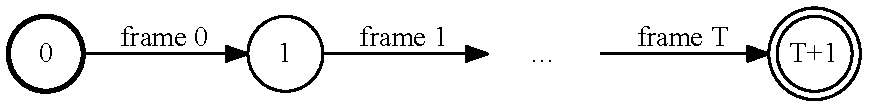
\includegraphics[scale=0.9]{img/t1.pdf}
\caption{{Weighted finite state transducer representing the input signal.}}
\label{fig:t1}
\end{figure}

\begin{figure}[ht]
\centering
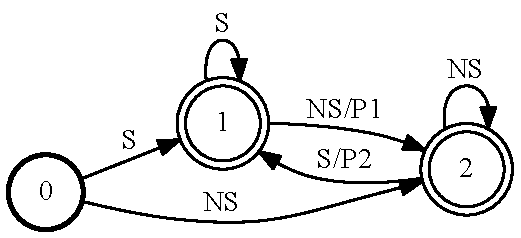
\includegraphics[scale=0.9]{img/t2.pdf}
\caption{{Weighted finite state transducer representing the basic smoothing model without any context for SAD.}}
\label{fig:t2}
\end{figure}

Given the two above described transducers, the decoding process is performed using on-the-fly composition of the transduction and the input model of an unknown size.
This is feasible since the input is considered to be a linear-topology, un-weighted, epsilon-free acceptor.
After each composition step, the shortest-path (considering tropical semiring) determined in the resulting model is compared with all other alternative hypotheses.
When a common path is found among these hypotheses (i.e., with the same output label), the corresponding concatenated output labels are marked as the final fixed output.
Since the rest of the best path is not certain, it is denoted as a temporary output (i.e., it can still be altered later in the process). 

The influence of smoothing the outputs of DNN on results can be observed in second row of Table~\ref{table:base} (+ Basic smoothing).
The results show an overall significant boost in all metrics.
For example, \mbox{F-value} improved from 0.3\% to 28.5\%, MR was reduced from 3.7\% to 2.2\%, and the value of $\delta_{2/3}$ improved noticeably from 0.42~s to 0.27~s.

\subsection{Using Artificial Training Data}
\label{ss:SADartificial}

The level of MR yielded so far (around 2\%) would still lead to a small increase in word error rate of the transcription system (e.g. from 13\% to 14\%) as the misclassified speech frames would be omitted from transcription. 
Upon closer inspection, most of the misclassified speech frames are segments with background noise.
This was caused by utilizing only speech data recorded in clean conditions (i.e., without any background noise) during DNN training.

To resolve this issue, training data containing various non-speech events in the background (e.g., music, jingles) were required.
Due to the lack of such annotated data, an artificial dataset created by mixing 30 hours of clean speech with non-speech recordings was constructed.
A larger set of non-speech recordings of a total length of 100 hours was prepared first.
After that, every speech recording was mixed with a randomly selected non-speech recording from the prepared set.
Note that every non-speech recording used for mixing had to have the same or longer duration than the given input speech recording (the selected non-speech recording was trimmed to match the length of the speech recording) and its volume was increased or decreased to match the desired level of SNR (which was also selected randomly from an interval between $-30$~dB and 50~dB).

The labels of this artificial data were created automatically. 
If SNR of a recording was higher than a defined threshold (0 dB), the recording was labeled as speech.
In the opposite case, the recording was annotated as non-speech.

The results are summarized in third row of Table~\ref{table:base} (+ Artificial training data).
It is evident that utilizing this artificial data led to an increase in F-measure and a significant reduction in MR from 2.2\% to 0.3\%.
Unfortunately, these improvements are all accompanied by an increase in FAR and, even more importantly, an increase in $\delta_{2/3}$ from 0.27~s to 0.34~s.
Due to these issues, a further refinement of the smoothing algorithm was investigated.

\subsection{Improved Context-Based Smoothing}
\label{ss:SADcontext}
The proposed refinement of the smoothing scheme is depicted in Fig.~\ref{fig:t3}.
In this case, both the speech and non-speech events are represented as sequences of three states, where the first and third states (the outer states) model the context.
Similarly to original smoothing model (i.e., without any context), the penalties are defined just for transitions between the speech and non-speech events, i.e., for transition a) from the end state of speech (\textit{end\_S}) to the start state of non-speech (\textit{start\_NS}), and b) from the end state of non-speech (\textit{end\_NS}) to the start state of speech (\textit{start\_S}).

\begin{figure}[ht]
\centering
	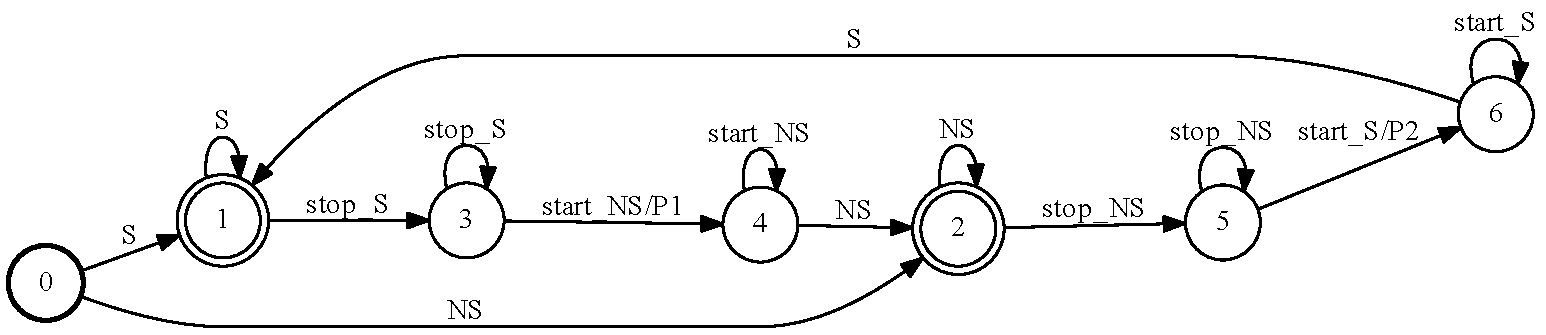
\includegraphics[scale=0.57]{img/cont.pdf}
\caption{{Weighted finite state transducer representing the context-based smoothing model for SAD.}}
\label{fig:t3}
\end{figure}

The training data from Sect.~\ref{ss:SADartificial} had to be modified to include transition between speech/non-speech events.
At first, two recordings were chosen randomly, one speech and one non-speech.
After that, these two recordings were concatenated in a random order.
The final recording then contained one of the two possible transitions (i.e., from speech to non-speech or from non-speech to speech) and was labeled automatically as follows:

\begin{enumerate}
	\item The number of transition frames was derived from the input feature context window (25-1-25).
	\item Only the 50 frames at the inner boundary of the two joined recordings were annotated as transitional, i.e., using 25 labels \textit{stop\_S} followed by 25 labels \textit{start\_NS} or 25 labels \textit{stop\_NS} followed by 25 labels \textit{start\_S}.
	\item All other frames were marked as either speech or non-speech.
\end{enumerate}

This approach, as the results show (see fourth row (Modified artificial data + context-based smoothing) in Table~\ref{table:base}), a) addresses the issue of an increase in $\delta_{2/3}$, which has emerged due to the use of the artificial training data, b) significantly decreases FAR and c) increases F-measure.
The value of $\delta_{2/3}$ was reduced from 0.34~s to 0.27~s.
The negligible downside is a slight increase in miss rate (by 0.2\%).

After achieving these satisfactory results, this speech activity detection approach was evaluated on standardized dataset.
% as well as integrated into TVR monitoring system to see its performance in real transcription system.

\subsection{Evaluation on QUT-NOISE-TIMIT Corpus} 
\label{ss:SADqut}

To compare the performance of the final proposed SAD approach (see Sect~\ref{ss:SADcontext}) with different approaches presented in literature, a standardized QUT-NOISE-TIMIT~\parencite{DBLP:conf/interspeech/DeanSVM10} corpus was utilized.
The comparison was done with five approaches already presented in~\parencite{DBLP:conf/interspeech/DeanSVM10} and two novel approaches with even better, state-of-the-art, results~\parencite{DBLP:conf/icassp/WisdomOAP15, DBLP:conf/interspeech/GhaemmaghamiDKS15}.

%A standardized QUT-NOISE-TIMIT~\parencite{DBLP:conf/interspeech/DeanSVM10} corpus is one of the very few corpora frequently used to compare the performance of various speech activity detection systems.
%It is suitable for training and evaluation of SAD systems in various SNR conditions.
%For these specific reasons, it was also used to evaluate the proposed SAD approach.

The five original SAD systems were: standardized VAD system ITU-T~G.729 Annex B~\parencite{qut-1}, standardized advanced front-end ETSI~\parencite{DBLP:conf/icassp/LiLWD04}, Sohn's likelihood ratio test~\parencite{DBLP:journals/spl/SohnKS99}, Ramirez's long-term spectral divergence (LTSD)~\parencite{DBLP:journals/speech/RamirezSBTR04} and GMM based approach with use of MFCC features~\parencite{DBLP:conf/interspeech/DeanSVM10}.
The newer approaches were voice activity detection using subband noncircularity (SNC)~\parencite{DBLP:conf/icassp/WisdomOAP15} and complete-linkage clustering (CLC) for VAD~\parencite{DBLP:conf/interspeech/GhaemmaghamiDKS15}.

\bigskip
\noindent
\textbf{QUT-NOISE-TIMIT Corpus}
\medskip

\noindent
As the authors stated, the main idea behind the creation of QUT-NOISE-TIMIT corpus~\parencite{DBLP:conf/interspeech/DeanSVM10} was a need for a standardized corpus for training and testing of speech activity detection in various target environments and in different SNR conditions.
For this purpose, they gathered more than 10 hours of background noise across 10 different unique locations to a corpus called QUT-NOISE.
These background noises covered five different but common scenarios (specifically cafe, home, street, car and reverb).
Each scenario was also composed of two different source locations:
\begin{itemize}
	\item cafe - outdoor cafe environment or indoor shopping food-court; 
	\item home - kitchen or living room;
	\item street - inner-city or outer-city traffic-light controlled intersections;
	\item car - windows down or up;
	\item reverb - indoor pool or partially enclosed carpark.
\end{itemize}	
The QUT-NOISE background noises were mixed with a clean speech from TIMIT corpus~\parencite{timit:1986} creating 600 hours of new recordings with various amount of speech segments, length (60 or 120 seconds) and SNR level ($-10$, $-5$, 0, 5, 10 or 15 dB).
These new recordings then formed the standardized QUT-NOISE-TIMIT corpus.
After that, the final corpus was evenly split into two groups (A and B) to provide training and testing subsets.

\bigskip
\noindent
\textbf{Evaluation Protocol}
\medskip

\noindent
The authors of QUT-NOISE-TIMIT also provided an evaluation protocol, which was than followed by others as well~\parencite{DBLP:conf/icassp/WisdomOAP15, DBLP:conf/interspeech/GhaemmaghamiDKS15}.
During the training phase, no information of target scenario was given to the system.
The only available prior knowledge was the SNR level of target environment: low noise (10,~15~dB), medium noise (0,~5~dB) or high noise ($-10$,~$-5$~dB).
For each of these target environments, group A was used for training and group B for testing and vice-versa.
The decoded segments were then compared with QUT-NOISE-TIMIT ground truth labels, and miss rate, false alarm rate and half-total error rate were evaluated (see Sect.~\ref{ss:SADmetrics}).

The proposed SAD approach followed this evaluation protocol, and it was trained as described in Sect.~\ref{ss:SADcontext}, of course, with the exception of not using the artificial training data (i.e., only the data from QUT-NOISE-TIMIT were utilized).
%Additionally, for each target SNR the performance of the proposed SAD approach in different scenarios was evaluated.

\bigskip
\noindent
\textbf{Low Noise Conditions}
\medskip

\noindent
The experiment in low noise conditions was based on recordings with SNR level of 10 and 15~dB.
The results are depicted in Fig.~\ref{fig:low}.
%The left part of the figure presents the comparison of various SAD systems.
As the results show, the proposed SAD approach outperformed all other systems by a fair margin.
The absolute reduction in HTER was more than~2\% over the second best complete-linkage clustering approach.
The achieved value of HTER was~2.6\%, the other metrics are given in first row of Table~\ref{table:qut}.
Note that the precision of the detected change points was also very good (F-value~85.1\% and $\delta_{2/3}$~0.05~s).
The proposed SAD approach thus achieved state-of-the-art results in low noise conditions.

\begin{table}
\caption{Performance of the proposed SAD approach on QUT-NOISE-TIMIT.}
\label{table:qut}
\centering
\begin{tabular}{lcccccc}
\hline
\noalign{\smallskip}
Conditions & HTER [\%] & FER [\%] & MR [\%] & FAR [\%] & F-value [\%] & $\delta_{2/3}$ [s] \\
\noalign{\smallskip}
\hline
\noalign{\smallskip}
Low noise & 2.7 & 2.6 & 2.2 & 3.0 & 85.1 & 0.05 \\
Medium n. & 5.8 & 5.8 & 5.8 & 5.8 & 65.2 & 0.11 \\
High n. & 17.0 & 16.4 & 24.0 & 10.0 & 33.1 & 0.22 \\
\hline
\end{tabular}
\end{table}

%The right side of the figure shows the performance of the proposed approach in all scenarios.
%The easiest scenarios in low noise conditions were scenarios car and street with only a small amount of errors.
%The most problematic scenarios were home (highest HTER) and reverb (a lot of missed speech forcing additional errors in transcription process).

\begin{figure}
\centering
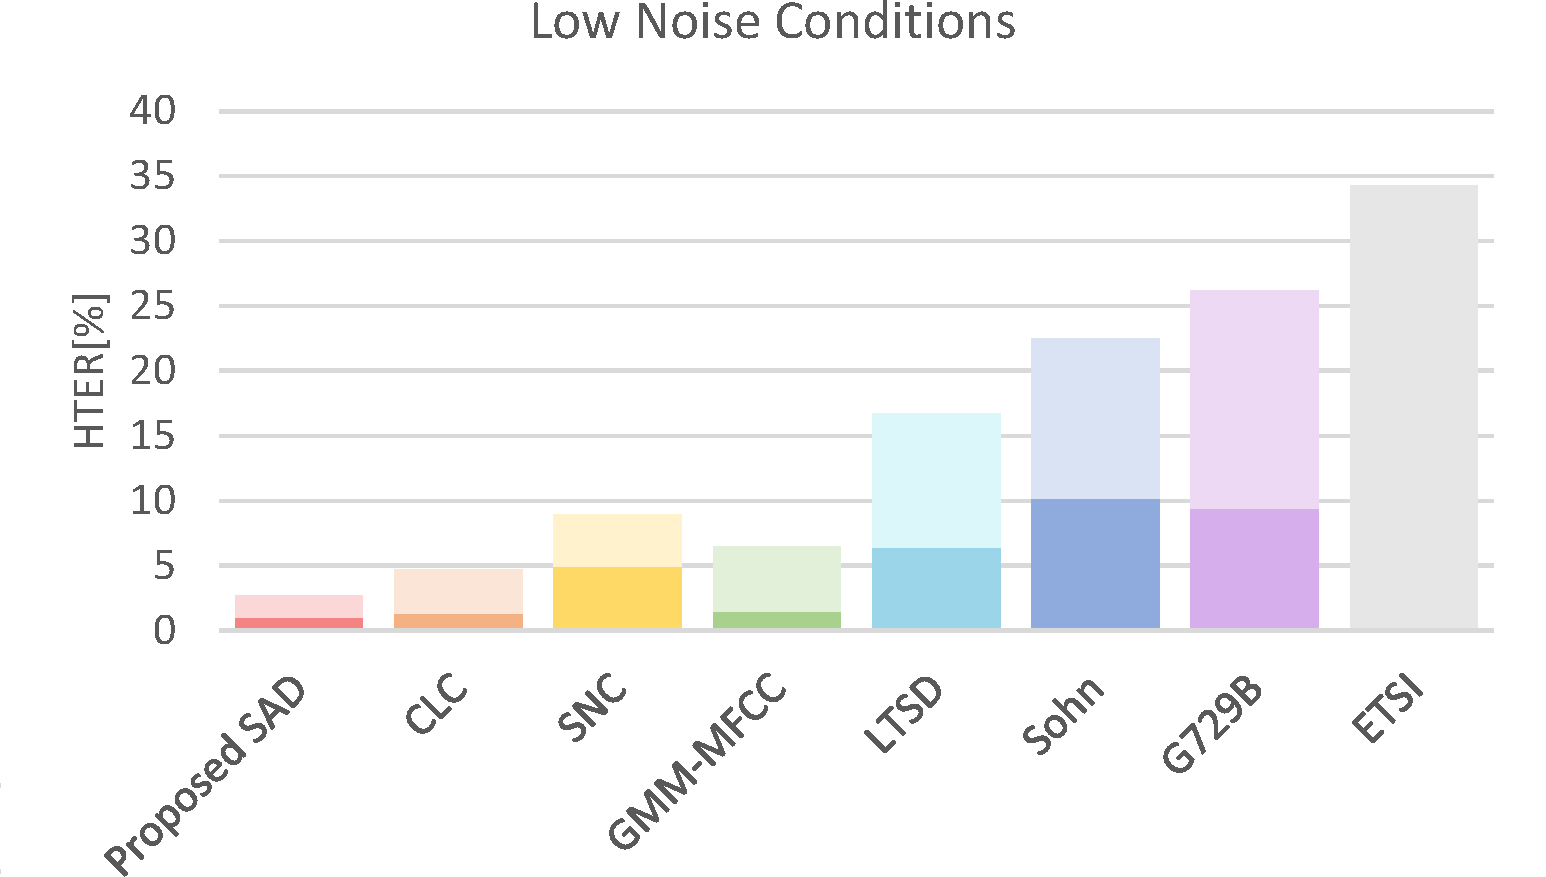
\includegraphics[scale=0.5]{img/gLow.pdf}
\caption{Comparison of results of various SAD approaches in low noise conditions on QUT-NOISE-TIMIT dataset. The contribution of MR and FAR to HTER bars is displayed by darker and lighter shades, respectively.}
\label{fig:low}
\end{figure}

\bigskip
\noindent
\textbf{Medium Noise Conditions}
\medskip

\noindent
Recordings with SNR level of~0 and 5~dB were utilized for experiment in medium noise conditions.
Figure~\ref{fig:med} depicts the results.
Similarly to experiment conducted in low noise conditions, the proposed SAD approach yielded the best results, outperformed the other systems and thus reached the state-of-the-art results.
Once again, the absolute reduction in HTER was over~2\% (the achieved value was 5.8\%, see second row of Table~\ref{table:qut}) over the second best CLC system.
The worsen conditions caused an increase of over~3\% in HTER for the proposed SAD approach.

%The right side of the Fig.~\ref{fig:med} compares the performance of the proposed approach in various scenarios.
%The car and street scenarios remained the least problematic (2-3\% in HTER) while cafe and reverb became the most troubling scenarios.
%Also note that reverb scenario resulted in most omitted speech causing worse speech transcription.

\begin{figure}
\centering
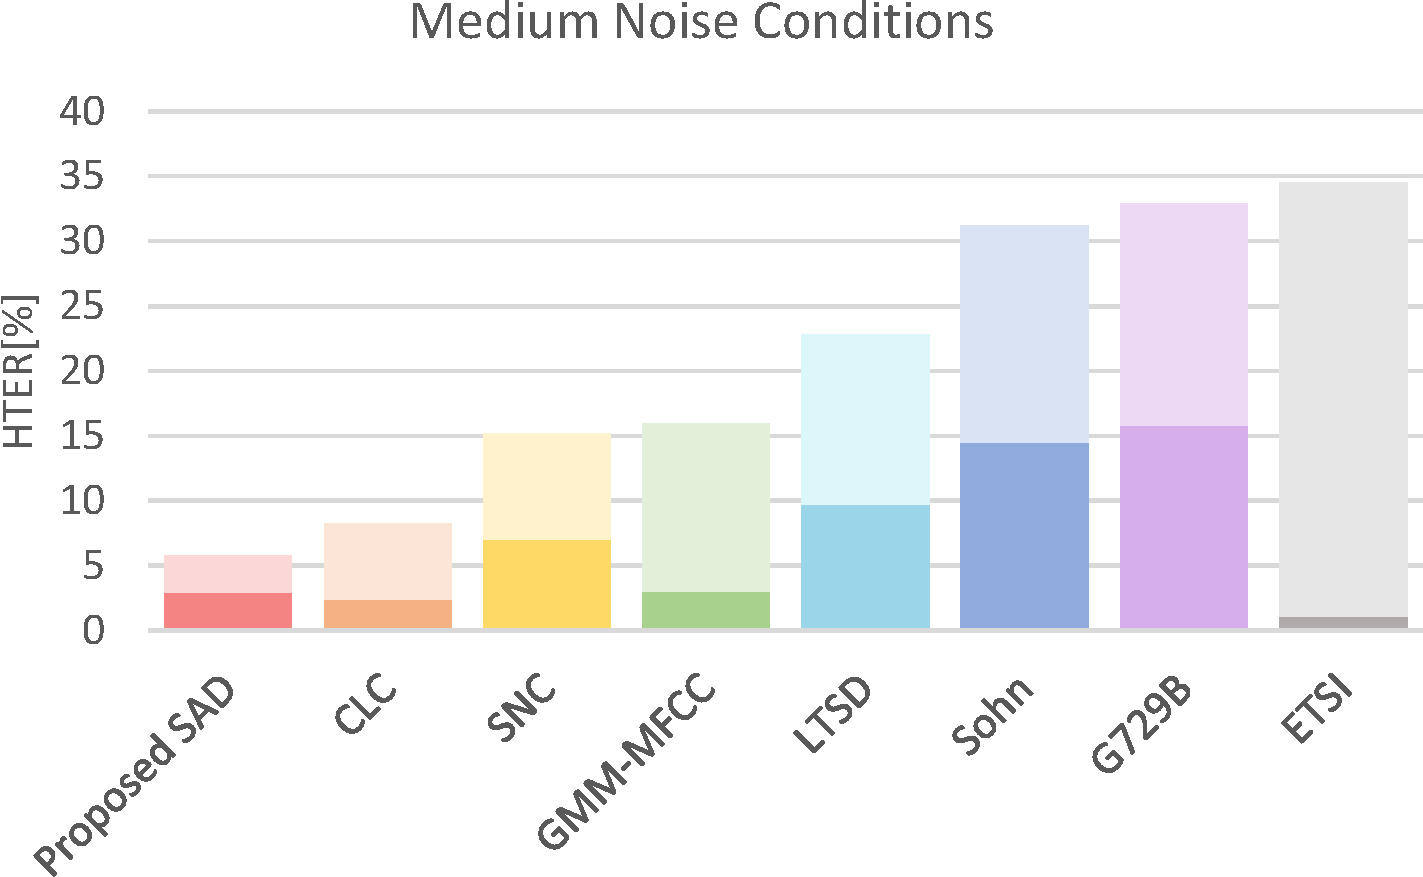
\includegraphics[scale=0.5]{img/gMedium.pdf}
\caption{Comparison of results of various SAD approaches in medium noise conditions on QUT-NOISE-TIMIT dataset. The contribution of MR and FAR to HTER bars is displayed by darker and lighter shades, respectively.}
\label{fig:med}
\end{figure}

\bigskip
\noindent
\textbf{Hard Noise Conditions}
\medskip

\noindent
The hardest conditions to segment were based on recordings with SNR level of~$-10$ and $-5$~dB.
The comparison of performance of various SAD systems is depicted in Fig.~\ref{fig:high}.
The proposed SAD approach was outperformed by approximately~2\% in HTER by complete linkage clustering.
However, it still outperformed the rest of the systems by a fair margin.
The achieved HTER was~17\% (an increase of over~11\% over the medium noise conditions).
The rest of the metrics are shown in third row of Table~\ref{table:qut}.
Unfortunately, most of its errors were caused by omitted speech (i.e., higher miss rate).
%and higher WER of speech transcription system).
%On the other hand, GMM-MFCC and ETSI systems had missed lower amount of speech making them slightly more suitable for further speech transcription.
However, the proposed SAD approach was not designed and fine-tuned for such low SNR conditions.

%The results of the proposed SAD approach in various scenarios are shown in Fig.~\ref{fig:high} (right section).
%The car scenario continued to be the easiest to segment (HTER slightly over~$5.5$\%) while the cafe and reverb scenarios remained the toughest ones (HTER close to~$28$\%).
%The reverb scenario was even harder as the most errors came from omitted speech making this scenario really hard to transcribe.

\begin{figure}
\centering
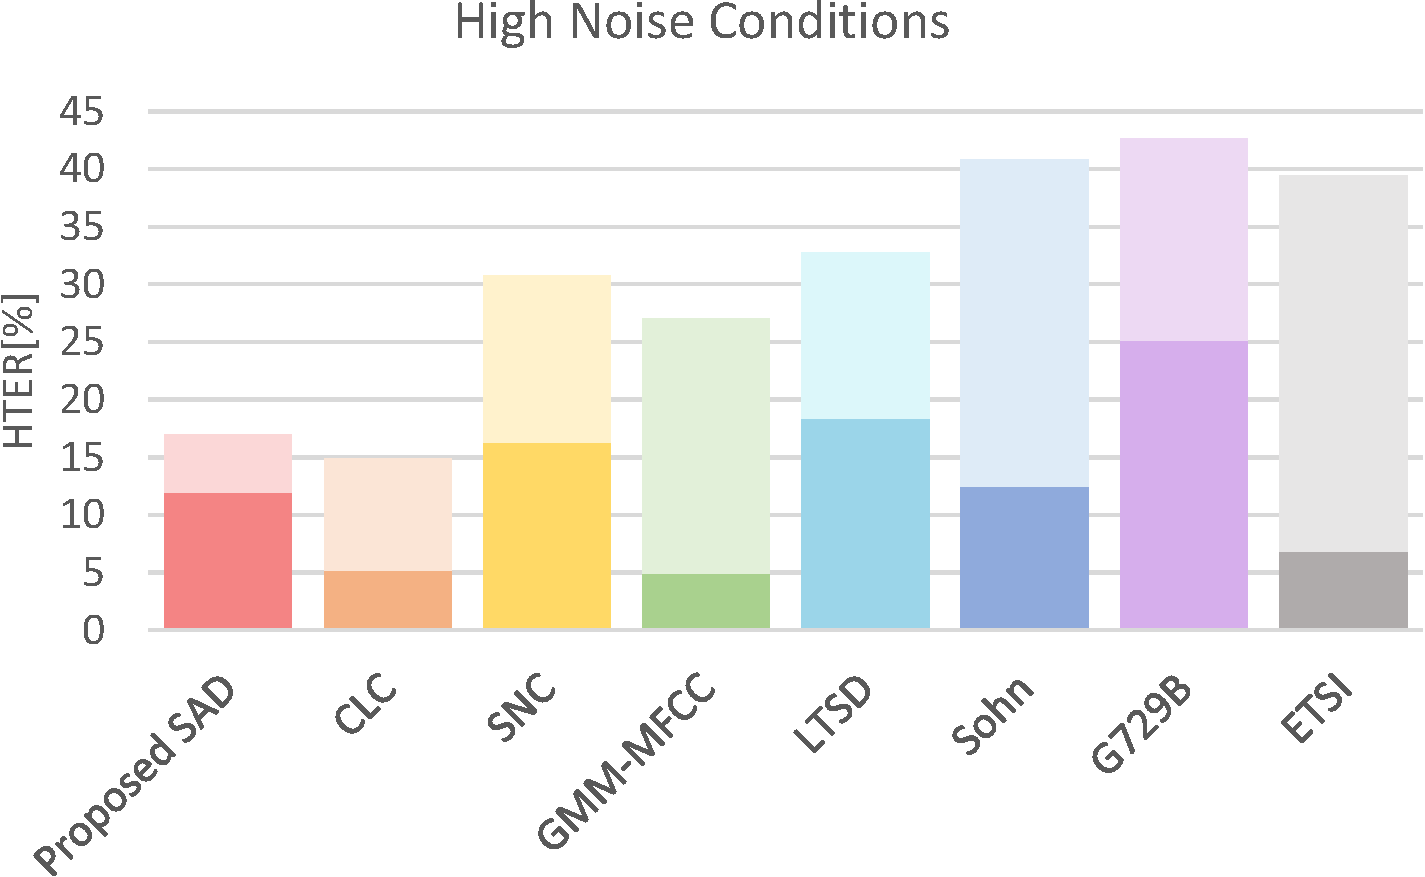
\includegraphics[scale=0.5]{img/gHigh.pdf}
\caption{Comparison of results of various SAD approaches in high noise conditions on QUT-NOISE-TIMIT dataset. The contribution of MR and FAR to HTER bars is displayed by darker and lighter shades, respectively.}
\label{fig:high}
\end{figure}

% \subsection{Tuning the Hyper-Parameters of DNN}
% \label{ss:SADhyper-parameters}

% \bigskip
% \noindent
% \textbf{The Importance of Local Normalization}
% \medskip

% \noindent
% All the concluded experiments utilized local mean normalization of input features within one second long window.
% The normalization process adds additional computational and time demands during the training and even evaluation phases.
% The goal of this experiment was thus to discard the local normalization in order to save processing time.
% Note that the hyper-parameters of DNN remained unchanged.

% Table~\ref{table:lN} presents the results of this experiment run a) with and b) without the local mean normalization.
% The results clearly show the necessity of applying this normalization as the results yielded without it are noticeably worse in every metric.
% The local mean normalization within 1 second window is thus an important part of the final speech activity detection module.

% \begin{table}
% \caption{Influence of no local normalization on results.}
% \label{table:lN}
% \centering
% \begin{tabular}{cccccc}
% \hline
% \noalign{\smallskip}
% Normalized & FER [\%] & MR [\%] & FAR [\%] & F-value [\%] & $\delta_{2/3}$ [s] \\
% \noalign{\smallskip}
% \hline
% \noalign{\smallskip}
% No & 3.4 & 0.8 & 10.0 & 35.6 & 0.29 \\
% Yes & 2.4 & 0.5 & 7.2 & 52.7 & 0.26 \\
% \hline
% \end{tabular}
% \end{table}

\subsection{Performance Details}
\label{ss:SADperformance}
A performance of the proposed speech activity detection approach was closely monitored so that it could be integrated into a real speech transcription system without any issues.
The proposed SAD approach averaged real-time factor of 0.01 and latency around 2 seconds (these values were measured using processor Intel Core i7-3770K @ 3.50GHz).
This performance allows for its seamless use in real-time processing without any major delay. 
% Given these values, the proposed SAD approach was then integrated into TVR monitoring system developed at SpeechLab@TUL, and it could be thus evaluated in a real speech transcription system.

\subsection{Evaluation of Proposed SAD Approach in a Real Speech Transcription System}
\label{ss:SADinST}
Given all the findings, results from previous experiments and fast performance, the final proposed speech activity detection approach (i.e., with context-based smoothing model) was integrated into TVR monitoring system developed at SpeechLab@TUL and thus evaluated in a real speech transcription system.

For this purpose, two test sets of Czech broadcasts were utilized (see Table~\ref{table:srData}).
The first set, recordings from local TV news channel, contained 22204 words, and approximately 60\% of its 4 hour length was labeled as speech.
The other set represented a local music radio station.
Its length was 8 hours (7212 words), and only 10\% of its content was considered as speech.

\begin{table}[ht]
\caption{Information about test sets for speech transcription.} 
\label{table:srData}
\centering
\begin{tabular}{lccr}
\hline
Test set & Duration & Speech [\%] & Words\\
\hline
Live news TV channel & 4 hours & 60\% & 22204\\
Local radio station & 8 hours & 10\% & 7212\\
\hline
\end{tabular}
\end{table}

The transcription system developed at SpeechLab@TUL employed an acoustic model based on a Hidden Markov Model - Deep Neural Network (HMM-DNN) hybrid architecture~\parencite{DBLP:journals/taslp/DahlYDA12}, where the baseline Gaussian Mixture Model (GMM) was trained as context-dependent, speaker-independent and contained 3886 physical states.
The acoustic model was trained on phonetically annotated 270 hours of clean speech recordings of Czech.
The hyper-parameters of DNN could be summed to:
\begin{itemize}
\item 5 hidden layers;
\item decreasing number of neurons per layer (1024-1024-768-768-512);
\item ReLU activation function;
\item mini-batches size of 1024;
\item learning rate 0.08;
\item 35 epochs.
\end{itemize}
The features were:
\begin{itemize}
\item 39-dimensional log filter banks;
\item concatenation of 5 previous frames, the current frame and 5 following frames;
\item local normalized within one-second window.
\end{itemize}
Note that fine-tuning of DNN hyper-parameters (used within this experiment) was published in~\parencite{ECMSM15} and later on further extended.

The linguistic part of the system was composed of a lexicon and a language model.
The lexicon contained 550,000 entries with multiple pronunciation variants and the language model was based on \mbox{N-grams}.
For practical reasons (mainly with respect to the very large vocabulary size), the system used bigrams.
However, 20 percent of all “word-pairs” actually included sequences containing three or more words, as the lexicon contains 4,000 multi-word collocations.
The unseen bigrams were backed-off by Kneser-Ney smoothing~\parencite{DBLP:conf/icassp/KneserN95}.

\bigskip
\noindent
\textbf{Experimental Results}
\medskip

\noindent
Within the scope of experimental evaluation, both test sets were transcribed a) with and b) without the use of the final speech activity detection approach.
The results are presented in Table~\ref{table:sr}, which contains values of word error rate and correctness (i.e., presents the accuracy of transcription). 
To measure computational demands with and without applying SAD, values of real-time factor are also presented.

\begin{table}[ht]
\caption{Evaluation of the proposed SAD approach in a real speech transcription system.} 
\label{table:sr}
\centering
\begin{tabular}{ccccc}
\hline
Test set & \multicolumn{2}{c}{live news TV channel} & \multicolumn{2}{c}{local radio station} \\
SAD module & Yes & No & Yes & No \\
\hline
WER [\%] & 12.4 & 12.7 & 14.0 & 17.9 \\
correctness [\%] & 89.7 & 89.7 & 88.5 & 88.4 \\
RTF & 0.42 & 0.77 & 0.08 & 0.83 \\
\hline
\end{tabular}
\end{table}

The results show that the utilization of the proposed speech activity detection approach was beneficial on both test sets.
The yielded improvements in WER and correctness proved that the proposed SAD approach omitted hardly any speech parts and even decreased the number of insertions (from non-speech parts).
The real-time factor was almost two times and more than ten times lower for local TV and radio broadcast test sets, respectively.
The decrease was, of course, more significant for the radio set because it contained significantly more non-speech events (e.g. music).
This resulted in huge savings in processing time and computational resources.

A small reminder, RTF of the proposed SAD approach is 0.01 and its latency is around 2 seconds (see Sect.~\ref{ss:SADperformance}).
Given these numbers and the fact that RTF of the transcription system is around 1, it's perfectly feasible to use the proposed speech activity detection approach in TVR monitoring system developed at SpeechLab@TUL without any major delay.

Thanks to all these findings, the proposed speech activity detection approach is also perfectly capable of working as the first phase of speaker change point detection to identify speech segments in recordings.
%Note that all the presented RTF values were measured using processor Intel Core i7-3770K @ 3.50GHz.

\section{Speaker Change Point Detection}
\label{ch:SCH}
The proposed speaker change point detection approach is also being designed in several consecutive steps.
These steps, from initial approach to the current one, are heavily discussed within this section.
The evaluation metrics and development data are also presented.
%At first, the evaluation metrics as well as development data are presented.
%After that, the individual consecutive steps from initial approach to the current one are discussed.

Note that the speech segments obtained by the proposed speech activity detection approach are utilized as inputs to speaker segmentation.

Also note that the speaker change point detection approach is still in development, and the first publication is planned for next year.

\subsection{Metrics Used for Evaluation}
\label{ss:SCHmetrics}
In total, 4 metrics (already presented for speech activity detection), were utilized to evaluate the performance of speaker change point detection.
Specifically, the metrics are precision, recall and derived from them, \mbox{F-value}.
Finally, the last metric is $\delta_{2/3}$.
The definitions and further information can be seen in Sect.~\ref{ss:SADmetrics} in Change Point Quality Measures paragraph.

\subsection{Data Used for Development}
\label{ss:SCHdata}
A small subset of standardized dataset COST278~\parencite{DBLP:conf/interspeech/ZibertMMMNFGDZPCZKTV05}, specifically Czech test data, was used for evaluation and development of speaker segmentation.
This test set consisted of four recordings of different Czech broadcasts (ČT1, Nova \& Prima) in a total length of hour and half.
It not only contained clean speech segments but also segments with background noise and jingles.
The annotations provided with COST278 dataset were utilized (these annotations can even be further used, e.g., for speaker verification \& identification tasks).
In total, there were 399 labeled transitions from one speaker to another.

\subsection{Baseline DNN-Based Approach with Smoothing}
\label{ss:SCHbaseline}
The baseline approach utilized a deep neural network as a binary classifier (change point/no change point) and weighted finite state transducers as a decoder to smooth the outputs of DNN.
The smoothing was integrated into the baseline approach straight away as it was necessary for proposed speech activity detection approach to yield at least decent results (as proved in Sect.~\ref{ss:SADsmoothing}).

A large dataset of manually annotated (or automatically annotated and corrected by hand) broadcasts of Czech TV/radio shows from 2009 to 2014 was utilized to extract training data.
In these broadcasts, transitions between two speakers were found and extracted (only if the duration of silence during the speaker transition was shorter than one second (longer silence should get detected by SAD)).
In total, 30 hours of recordings (with the average length of one recording being around 5 seconds) were gathered.
This resulted in 20,000 speaker transitions, which could be divided into 4 groups (the transition from female to female, female to male, male to female and male to male) each represented by 5,000 change points.

The annotations for this extracted data were generated in an automated way.
The frame corresponding to the actual change point as well as safety collar frames around it were labeled as change point.
This safety collar was set to 1 second (100 frames).
This is due to the fact that determining the precise change point is quite often an ambiguous task (silence, crosstalk, etc.), and to provide the network with more information about the transition from one speaker to another.
The rest of the recording was labeled as segments without transition.
The annotation of one recording is depicted in Fig.~\ref{fig:SCP}.

\begin{figure}[ht]
\centering
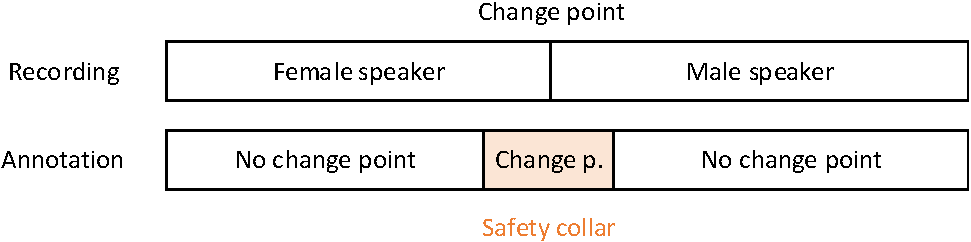
\includegraphics[scale=0.8]{img/scp-data.pdf}
\caption{{Example of annotation of recording from training data for SCP.}}
\label{fig:SCP}
\end{figure}

The hyper-parameters of deep neural network utilizing this data were set to:
\begin{itemize}
	\item 2 hidden layers;
	\item 64 neurons per hidden layer;
	\item ReLU activation function;
	\item mini-batches size of 1024;
	\item 0.08 learning rate;
	\item 15 epochs.
\end{itemize}
The extracted features were:
\begin{itemize}
	\item 39-dimensional log filter banks; 
	\item concatenation of 100 previous frames, the current frame and 100 following frames;
	\item no local normalized.
\end{itemize}

The decoding was done as described in Sect~\ref{ss:SADsmoothing} with the exception of applying different transduction model (slightly modified to be more suitable for speaker change point detection).
This transduction model (depicted in Fig.~\ref{fig:SCH1}) consists of two states (denoted 0 and 1).
The transitions between states 0/1 emit labels start/end change point with a time mark.
The final change points are then in the middle of start and end change point time marks.
The transitions are also weighted by penalty factors P1 and P2.
Note that their values (25 and 25) were tuned on different dataset.

\begin{figure}[ht]
\centering
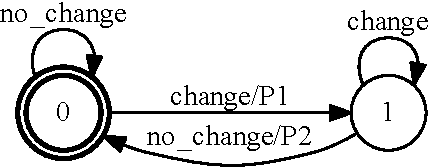
\includegraphics[scale=0.9]{img/SCH1.pdf}
\caption{{Weighted finite state transducer representing the basic smoothing model for SCP.}}
\label{fig:SCH1}
\end{figure}

The results of the baseline approach are summarized in first row of Table~\ref{table:baseSCH}.
The achieved results provide a decent starting point, but especially the precision is not particularly good.
This resulted in a need of different transduction model, which would be more suitable for the task of speaker segmentation.

\begin{table}
\caption{Summarized results of the proposed SCP approach described in Sect.~\ref{ch:SCH}.} \label{table:baseSCH}
\centering
\begin{tabular}{lcccc}
\hline
\noalign{\smallskip}
 Approach & Precision [\%] & Recall [\%] & F-value [\%] & $\delta_{2/3}$ [s] \\
\noalign{\smallskip}
\hline
\noalign{\smallskip}
 Baseline DNN-based & \multirow{2}{*}{46.9} & \multirow{2}{*}{72.8} & \multirow{2}{*}{57.1} & \multirow{2}{*}{0.23} \\
 + Basic smoothing &&&& \\
 + Forced duration smoothing & 48.7 & 76.0 & 59.3 & 0.22 \\
 + Artificial data & 65.4 & 73.9 & 69.4 & 0.20 \\
\hline
\end{tabular}
\end{table}

\subsection{Improved Smoothing with Forced Duration}
\label{ss:SCHforced}
The improved smoothing scheme was designed to reflect the annotation style of training data and fit the task of speaker change point detection more.
As described in previous section, 1 second long window (100 frames) around the actual change point was labeled as change point during the training.
However, during the decoding, the duration of the transition between speakers was decided by the decoder itself and varied greatly.
Within this experiment, the duration of this transition was forced to be precisely 1 second.

To reflect this concept, the transduction model had to be modified.
The new scheme is depicted in Fig.~\ref{fig:SCH3}.
The model consists of two main states (0 and 1) and 98 forced transition states (depicted as \dots; the number of the states corresponds to the forced duration of the transition).
When a transition from one speaker to another happens, the decoder has to go from state 0 through transition states to state 1; the change point label is output here; and back through the rest of the transition states to state 0, where it idles until next transition happens.
The transitions are as usual penalized by factors P1 and P2 (weights being set to 25 and 25).

\begin{figure}[ht]
\centering
	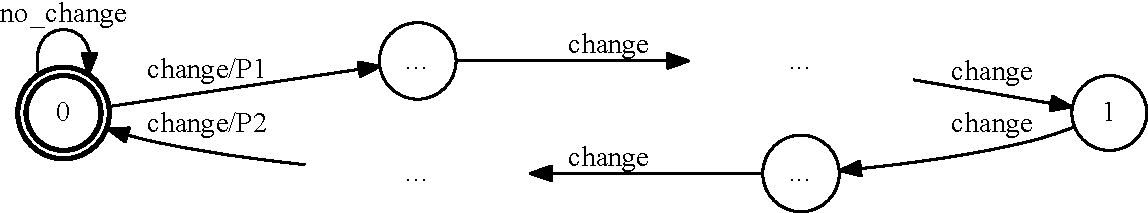
\includegraphics[scale=0.75]{img/SCH2.pdf}
\caption{{Weighted finite state transducer representing the smoothing model with forced duration for SCP.}}
\label{fig:SCH3}
\end{figure}

%\begin{figure}[ht]
%\centering
%	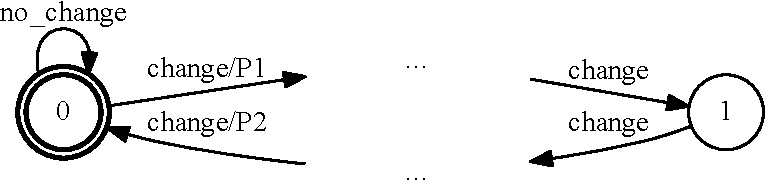
\includegraphics[scale=0.9]{img/SCH3.pdf}
%\caption{{Weighted finite state transducer representing the smoothing model with forced duration for SCP.}}
%\label{fig:SCH3}
%\end{figure}

The results are presented in second row of Table~\ref{table:baseSCH} (+ Forced duration smoothing).
An overall slight improvement in all observed  metrics was achieved (e.g. \mbox{F-value} increased from 57.1\% to 59.3\%).
However, the results could still be hugely improved.

\subsection{Adding Artificial Data}
\label{ss:SCHartificial}
After evaluating the performance of the proposed approach on selected recordings (from different dataset), two types of errors were more prominent.
The first common error was caused by quick transitions between speakers (without any silence) usually caused by artificial cuts (e.g. in news).
These change points got consistently ignored by the decoder.
The other common issue were longer silences (more than 0.5 s) in a speaker homogeneous segments.
These longer silences were usually caused by a deep breath or hesitation, and they forced the decoder to output a false speaker change point.
This issue is not that problematic as it could be fixed later on with speaker clustering.
However, both of these errors boil down to the fact that the deep neural network did not see such data during training.

For this reason, the training data presented in Sect.~\ref{ss:SCHbaseline} was enriched by 20 additional hours.
To deal with the first issue, approximately 10 hours of recordings containing quick cuts between speakers were prepared by artificially joining recordings of different speakers in quick succession.
The labels were generated in the same way as for the original data.
In total, 14,340 transitions were added to DNN training with uniform distribution between transition types (female-female, female-male, male-female, male-male).
To solve the second issue, 10 hours of speaker homogeneous segments (including longer silences) were added to training. 
This whole 10 hours were labeled as segments with no change point.
Within this experiment, DNN and WFST remained the same as presented in previous sections.

By utilizing this additional data, the results improved significantly (see third row of Table~\ref{table:baseSCH}).
The precision of change point detection increased from 48.7\% to 65.4\%, \mbox{F-value} got boosted from 59.3\% to 69.4\%, and even the speaker change point placement improved ($\delta_{2/3}$ was reduced from 0.22 s to 0.2 s).
The only downside is a small decrease in recall (approximately 2\%).
However, this issue is easily overweighted by the overall improvements.

Even though the results improved significantly, there is still a room for further improvements before integrating the speaker change point detection into TVR monitoring system developed at SpeechLab@TUL.
The design of the SCP approach is still being researched.
As of right now, the results are fairly comparable with LIUM Speaker Diarization toolkit (without clustering).

\chapter{Conclusions}
\label{ch:conclusions}

This thesis statement presents the current progress of final thesis focused on a task of speaker change point detection.
The main goal is/was to design a novel approach based on state-of-the-art technologies (namely DNNs), which can be integrated into existing TVR monitoring system developed at SpeechLab@TUL.
For this reason, it has to support an online mode operating with low latency to process real-time streams.
The final speaker segmentation operates in two consecutive phases:

\begin{itemize}
	\item Speech Activity Detection - \textbf{completed and published}
	
	The proposed speech activity detection approach is based on feed-forward deep neural network and weighted finite state transducers.
	The DNN is used as a speech/non-speech classifier, while the context-based WFST decoder smooths the outputs.
	The network is trained on data artificially created by mixing speech and non-speech recordings at various levels of SNR.
	This design yields state-of-the-art results in low and medium noise conditions on standardized QUT-NOISE-TIMIT dataset.
	It is also suitable for online use as it operates with low real-time factor as well as low latency.

	The proposed speech activity detection approach is now fully integrated into the TVR monitoring system developed at SpeechLab@TUL.
	Last month, approximately 4,130 days (99,100 hours or 2.3TB) of recordings were transcribed in processing time of 1,333 days (32,000 hours).
	Considering the real-time factor of the speech transcriber is around 1, the utilization of SAD as preprocessor resulted in a significant saving of processing time.
	Approximately two thirds of data was non-speech segments, and it was thus omitted from transcription.
	This omission also resulted in slight increase of accuracy of the system as the non-speech parts were not transcribed into jibberish.

	The initial research introducing the main idea and basic smoothing model was presented in~\parencite{SIGMAP16} at SIGMAP 2016 held in Lisbon.
	The improved context-based smoothing model, which yields state-of-the-art results, was introduced in~\parencite{ICASSP17} at ICASSP 2017 conference in New Orleans.
	Finally, an extended version of this work presenting more experiments and in detail evaluation on QUT-NOISE-TIMIT was published in~\parencite{SPRINGER17}.
	The papers also reported the benefits of employing the proposed speech activity detection approach in conjunction with speech recognizer.
	
	The proposed speech activity detection approach follows all the set goals, and it is now considered as fully completed.
	
	\item Speaker Change Point Detection - \textbf{in progress}
	
	The speaker change point detection approach is in early stage of development.
	The current approach utilizes feed-forward deep neural network as classifier and weighted finite state transducers (with forced duration of transition) as decoder to mark the transitions between two speakers.
	The network is trained on a mixture of real and artificially mixed broadcast data of Czech TV/radio shows.
	% As of right now, the proposed transducer distinguishes between four different transitions (female-female, female-male, male-female, male-male) and is trained on Czech broadcasts. 
	It is also possible to use it for online streams as it operates with low latency \& real-time factor.
	The achieved results are promising, but they still leave much to be desired.
	Further research is thus required.
	
	The further research will be focused on different input feature vectors as the log filter banks may not contain all the necessary information to distinguish between speakers.
	Features, such as i-vectors, d-vectors, etc., could be employed to improve the results.
	Another possibility, as the literature suggests, is to employ different, more complex, classifier, such as convolutional or long short term memory recurrent neural networks (bidirectional).
	It is also possible to further tune WFST transduction scheme (e.g. to distinguish between four different transitions (female-female, female-male, male-female, male-male)).
	A mixture of more complex features \& classifier with WFST-based decoder should yield better results.
	
	The plan is to get the first paper published in 2018. 
	The final proposed speaker segmentation approach (fulfilling all the set goals) will be then integrated into TVR monitoring system developed at SpeechLab@TUL.
	It will provide the monitoring system with functionality of detecting speaker homogeneous segments.
		
\end{itemize}	

%The main contribution of this thesis lies in:
%\begin{itemize}
%	\item a proposed approach for speaker segmentation, that operates in two consecutive phases (speech activity detection and speaker change point detection),
%	\item robust speech activity detection approach, that utilizes DNNs and WFST to achieve state-of-the-art results on QUT-NOISE-TIMIT dataset, and also saves processing time and reduces WER of speech transcriber,
%	\item speaker change point detection approach (based on state-of-the-art technologies), that finds speaker homogeneous segments,
%	%\item at least comparative results with already existing methods,
%	\item online mode operating with low latency and real-time factor to process real-time streams,
%	\item integration of proposed approach into existing TVR monitoring system,
%	\item publications at international conferences.
%\end{itemize}	

%The fully integrated speaker change point detection approach can be then used as a starting point for future speaker verification \& identification systems.
%The speaker homogeneous segments can be complemented with additional information such as language or gender.
%A language identification approach distinguishing between 11 Slavic languages based on deep neural networks and weighted finite state transducers is already finished.
%It employs state-of-the-art bottleneck features extracted from DNN trained to predict senone posteriors.
%The paper should get published in 2018.
%The speaker homogeneous segments can also be used for research in field of speaker adaptive training for speech recognition to improve the performance of transcriber of SpeechLab@TUL even further.

%The language identification module is still in the works.
%The focus is on distinguishing between 11 Slavic languages (Czech, Slovak, Polish, Russian, Slovene, Ukrainian, Serbian, Macedonian, Croatian, Belarusian and Bulgarian) which could help a) with further segmentation, and b) to obtain more training data for acoustic models for speech recognizer.
	
%A similar approach to speech activity detection is applied.
%It is once more based on deep neural networks and weighted finite state transducers.
%However, instead of employing traditional features (log filter banks), state-of-the-art bottleneck features extracted from DNN trained to predict senone posteriors as suggested in~\parencite{DBLP:conf/interspeech/RichardsonRD15, DBLP:conf/icassp/McLarenFL16, DBLP:journals/taslp/FerrerLMS16} are used.
%A baseline module using i-vectors~\parencite{DBLP:conf/interspeech/MartinezPBGM11} is trained as well.

%The research should get published during next year.

% reference
\addcontentsline{toc}{chapter}{References}
\printbibliography[title=References]
%\bibliography{references}

% seznam publikací
\newpage
\chapter*{Author's Publications}
\addcontentsline{toc}{chapter}{Author's Publications}

\textbf{2017:}
	\begin{enumerate}[leftmargin=*]
		\bibitem{SPRINGER2017}
		Mateju L., P. Cerva, and J. Zdansky (2017). “Investigation into the Use of WFSTs and DNNs for 
		Speech Activity Detection in Broadcast Data Transcription”. In: \textit{E-Business and
		Telecommunications - 13th International Joint Conference, ICETE 2016, Lisbon,
		Portugal, July 26-28, 2016, Revised Selected Papers}, pp. 341–358.
	
		\bibitem{TSD2017}
		Safarik R. and L. Mateju (2017). “The Impact of Inaccurate Phonetic Annotations 
		on Speech Recognition Performance”. In: \textit{Text, Speech, and Dialogue - 20th 
		International Conference, TSD 2017, Prague, Czech Republic, August 27-31, 2017, 
		Proceedings}, pp. 402–410.
	
		\bibitem{ICASSP2017}
		Mateju L., P. Cerva, J. Zdansky, and J. Malek (2017). “Speech Activity Detection in 
		Online Broadcast Transcription Using Deep Neural Networks and Weighted Finite
		State Transducers”. In: \textit{2017 IEEE International Conference on Acoustics, Speech 
		and Signal Processing, ICASSP 2017, New Orleans, LA, USA, March 5-9, 2017}, 
		pp. 5460–5464.
	\end{enumerate}
	
	\noindent \textbf{2016:}
	\begin{enumerate}[leftmargin=*,resume]
		\bibitem{TSD2016}
		Bohac M., L. Mateju, M. Rott, and R. Safarik (2016). “Automatic Syllabification and 
		Syllable Timing of Automatically Recognized Speech - for Czech”. In: \textit{Text, Speech, 
		and Dialogue - 19th International Conference, TSD 2016, Brno, Czech Republic, 
		September 12-16, 2016, Proceedings}, pp. 540–547.
	
		\bibitem{SIGMAP2016}
		Mateju L., P. Cerva, and J. Zdansky (2016). “Study on the Use of Deep Neural Networks 
		for Speech Activity Detection in Broadcast Recordings”. In: \textit{Proceedings of the 13th 
		International Joint Conference on e-Business and Telecommunications (ICETE 
		2016) - Volume 5: SIGMAP, Lisbon, Portugal, July 26-28, 2016}, pp. 45–51.
		
		\bibitem{TSP2016}
		Safarik R. and L. Mateju (2016). “Impact of Phonetic Annotation Precision on Automatic 
		Speech Recognition Systems”. In: \textit{39th International Conference on 
		Telecommunications and Signal Processing, TSP 2016, Vienna, Austria, June 27-29, 2016}, 
		pp. 311–314.
	\end{enumerate}
	
	\noindent \textbf{2015:}
	\begin{enumerate}[leftmargin=*,resume]
		\bibitem{ECMSM2015}
		Mateju L., P. Cerva, and J. Zdansky (2015). “Investigation into the Use of Deep Neural 
		Networks for LVCSR of Czech”. In: \textit{2015 IEEE International Workshop of Electronics, 
		Control, Measurement, Signals and their Application to Mechatronics, ECMSM, 
		2015, Liberec, Czech Republic, June 22-24, 2015}, pp. 184–187.
	\end{enumerate}
	
	% \textbf{2017:}
	% \begin{enumerate}[leftmargin=*]
		% \bibitem{SPRINGER2017}
		% L. Mateju, P. Cerva, and J. Zdansky, “Investigation into the Use of WFSTs and DNNs for 
		% Speech Activity Detection in Broadcast Data Transcription,” in \textit{E-Business and
		% Telecommunications - 13th International Joint Conference, ICETE 2016, Lisbon,
		% Portugal, July 26-28, 2016, Revised Selected Papers}, pp. 341–358, 2017.
	
		% \bibitem{TSD2017}
		% R. Safarik and L. Mateju, “The Impact of Inaccurate Phonetic Annotations 
		% on Speech Recognition Performance,” in \textit{Text, Speech, and Dialogue - 20th 
		% International Conference, TSD 2017, Prague, Czech Republic, August 27-31, 2017, 
		% Proceedings}, pp. 402–410, 2017.
	
		% \bibitem{ICASSP2017}
		% L. Mateju, P. Cerva, J. Zdansky, and J. Malek, “Speech Activity Detection in 
		% Online Broadcast Transcription Using Deep Neural Networks and Weighted Finite
		% State Transducers,” in \textit{2017 IEEE International Conference on Acoustics, Speech 
		% and Signal Processing, ICASSP 2017, New Orleans, LA, USA, March 5-9, 2017}, 
		% pp. 5460–5464, 2017.
	% \end{enumerate}
	
	% \noindent \textbf{2016:}
	% \begin{enumerate}[leftmargin=*,resume]
		% \bibitem{TSD2016}
		% M. Bohac, L. Mateju, M. Rott, and R. Safarik, “Automatic Syllabification and 
		% Syllable Timing of Automatically Recognized Speech - for Czech,” in \textit{Text, Speech, 
		% and Dialogue - 19th International Conference, TSD 2016, Brno, Czech Republic, 
		% September 12-16, 2016, Proceedings}, pp. 540–547, 2016.
	
		% \bibitem{SIGMAP2016}
		% L. Mateju, P. Cerva, and J. Zdansky, “Study on the Use of Deep Neural Networks 
		% for Speech Activity Detection in Broadcast Recordings,” in \textit{Proceedings of the 13th 
		% International Joint Conference on e-Business and Telecommunications (ICETE 
		% 2016) - Volume 5: SIGMAP, Lisbon, Portugal, July 26-28, 2016}, pp. 45–51, 
		% 2016.
		
		% \bibitem{TSP2016}
		% R. Safarik and L. Mateju, “Impact of Phonetic Annotation Precision on Automatic 
		% Speech Recognition Systems,” in \textit{39th International Conference on 
		% Telecommunications and Signal Processing, TSP 2016, Vienna, Austria, June 27-29, 2016}, 
		% pp. 311–314, 2016.
	% \end{enumerate}
	
	% \noindent \textbf{2015:}
	% \begin{enumerate}[leftmargin=*,resume]
		% \bibitem{ECMSM2015}
		% L. Mateju, P. Cerva, and J. Zdansky, “Investigation into the Use of Deep Neural 
		% Networks for LVCSR of Czech,” in \textit{2015 IEEE International Workshop of Electronics, 
		% Control, Measurement, Signals and their Application to Mechatronics, ECMSM, 
		% 2015, Liberec, Czech Republic, June 22-24, 2015}, pp. 184–187, 2015.
	% \end{enumerate}
	
\end{document}
